
\section{System overview}\label{sec:sysoverview}

In conjunction with the start of this thesis a system sketch of Comordo's planned recommender system was given, shown in \figureref{fig:sysoverview}. The system consists of several parts surrounding the recommendation algorithms as it's core.

\vspace{-0.3cm}
\begin{figure}[h!]
  \centering
    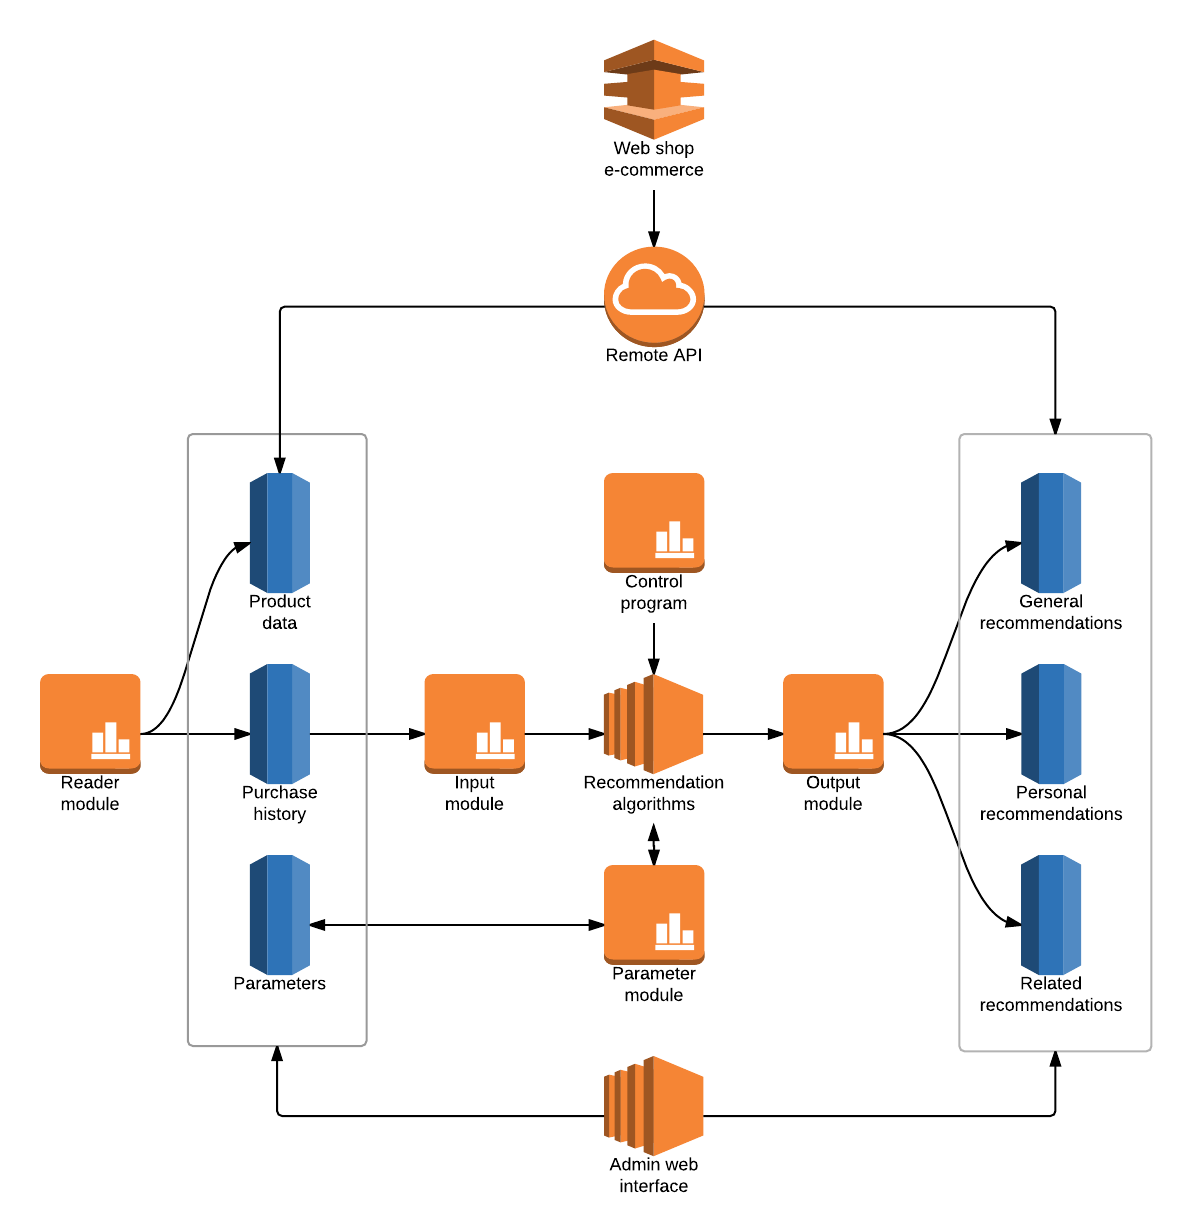
\includegraphics[width=0.9\textwidth]{fig/system_overview.png}
  \caption{Commordo's system sketch}
  \label{fig:sysoverview}
\end{figure}

\FloatBarrier

\begin{description}
    \item[Reader module] is responsible for reading data files provided by Commordo's clients.
    \item[Input module] provides the algorithms with transformed data.
    \item[Output module] populates the database with recommendations.
    \item[Control program] handles learning and optimization of the algorithms.
    \item[Parameter module] stores and adjusts parameters the algorithms use.
    \item[Remote API] is a REST based API, the endpoint for Commordo's clients.
    \item[Admin web interface] is a user friendly way for e-commerce clients to customize system settings and view recommendations.
\end{description}

